\documentclass[a4paper, 11pt]{report}

\input{../../../latex_template/preamble}
%From M275 "Topology" at SJSU
\newcommand{\id}{\mathrm{id}}
\newcommand{\taking}[1]{\xrightarrow{#1}}
\newcommand{\inv}{^{-1}}

%From M170 "Introduction to Graph Theory" at SJSU
\DeclareMathOperator{\diam}{diam}
\DeclareMathOperator{\ord}{ord}
\newcommand{\defeq}{\overset{\mathrm{def}}{=}}

%From the USAMO .tex files
\newcommand{\ts}{\textsuperscript}
\newcommand{\dg}{^\circ}
\newcommand{\ii}{\item}

% % From Math 55 and Math 145 at Harvard
% \newenvironment{subproof}[1][Proof]{%
% \begin{proof}[#1] \renewcommand{\qedsymbol}{$\blacksquare$}}%
% {\end{proof}}

\newcommand{\liff}{\leftrightarrow}
\newcommand{\lthen}{\rightarrow}
\newcommand{\opname}{\operatorname}
\newcommand{\surjto}{\twoheadrightarrow}
\newcommand{\injto}{\hookrightarrow}
\newcommand{\On}{\mathrm{On}} % ordinals
\DeclareMathOperator{\img}{im} % Image
\DeclareMathOperator{\Img}{Im} % Image
\DeclareMathOperator{\coker}{coker} % Cokernel
\DeclareMathOperator{\Coker}{Coker} % Cokernel
\DeclareMathOperator{\Ker}{Ker} % Kernel
\DeclareMathOperator{\rank}{rank}
\DeclareMathOperator{\Spec}{Spec} % spectrum
\DeclareMathOperator{\Tr}{Tr} % trace
\DeclareMathOperator{\pr}{pr} % projection
\DeclareMathOperator{\ext}{ext} % extension
\DeclareMathOperator{\pred}{pred} % predecessor
\DeclareMathOperator{\dom}{dom} % domain
\DeclareMathOperator{\ran}{ran} % range
\DeclareMathOperator{\Hom}{Hom} % homomorphism
\DeclareMathOperator{\Mor}{Mor} % morphisms
\DeclareMathOperator{\End}{End} % endomorphism

\newcommand{\eps}{\epsilon}
\newcommand{\veps}{\varepsilon}
\newcommand{\ol}{\overline}
\newcommand{\ul}{\underline}
\newcommand{\wt}{\widetilde}
\newcommand{\wh}{\widehat}
\newcommand{\vocab}[1]{\textbf{\color{blue} #1}}
\providecommand{\half}{\frac{1}{2}}
\newcommand{\dang}{\measuredangle} %% Directed angle
\newcommand{\ray}[1]{\overrightarrow{#1}}
\newcommand{\seg}[1]{\overline{#1}}
\newcommand{\arc}[1]{\wideparen{#1}}
\DeclareMathOperator{\cis}{cis}
\DeclareMathOperator*{\lcm}{lcm}
\DeclareMathOperator*{\argmin}{arg min}
\DeclareMathOperator*{\argmax}{arg max}
\newcommand{\cycsum}{\sum_{\mathrm{cyc}}}
\newcommand{\symsum}{\sum_{\mathrm{sym}}}
\newcommand{\cycprod}{\prod_{\mathrm{cyc}}}
\newcommand{\symprod}{\prod_{\mathrm{sym}}}
\newcommand{\Qed}{\begin{flushright}\qed\end{flushright}}
\newcommand{\parinn}{\setlength{\parindent}{1cm}}
\newcommand{\parinf}{\setlength{\parindent}{0cm}}
% \newcommand{\norm}{\|\cdot\|}
\newcommand{\inorm}{\norm_{\infty}}
\newcommand{\opensets}{\{V_{\alpha}\}_{\alpha\in I}}
\newcommand{\oset}{V_{\alpha}}
\newcommand{\opset}[1]{V_{\alpha_{#1}}}
\newcommand{\lub}{\text{lub}}
\newcommand{\del}[2]{\frac{\partial #1}{\partial #2}}
\newcommand{\Del}[3]{\frac{\partial^{#1} #2}{\partial^{#1} #3}}
\newcommand{\deld}[2]{\dfrac{\partial #1}{\partial #2}}
\newcommand{\Deld}[3]{\dfrac{\partial^{#1} #2}{\partial^{#1} #3}}
\newcommand{\lm}{\lambda}
\newcommand{\uin}{\mathbin{\rotatebox[origin=c]{90}{$\in$}}}
\newcommand{\usubset}{\mathbin{\rotatebox[origin=c]{90}{$\subset$}}}
\newcommand{\lt}{\left}
\newcommand{\rt}{\right}
\newcommand{\bs}[1]{\boldsymbol{#1}}
\newcommand{\exs}{\exists}
\newcommand{\st}{\strut}
\newcommand{\dps}[1]{\displaystyle{#1}}

\newcommand{\sol}{\setlength{\parindent}{0cm}\textbf{\textit{Solution:}}\setlength{\parindent}{1cm} }
\newcommand{\solve}[1]{\setlength{\parindent}{0cm}\textbf{\textit{Solution: }}\setlength{\parindent}{1cm}#1 \Qed}

\DeclareMathOperator{\sech}{sech}
\DeclareMathOperator{\csch}{csch}
\DeclareMathOperator{\arcsec}{arcsec}
\DeclareMathOperator{\arccsc}{arccsc}
\DeclareMathOperator{\arccot}{arccot}
\DeclareMathOperator{\arsinh}{arsinh}
\DeclareMathOperator{\arcosh}{arcosh}
\DeclareMathOperator{\artanh}{artanh}
\DeclareMathOperator{\arcsch}{arcsch}
\DeclareMathOperator{\arsech}{arsech}
\DeclareMathOperator{\arcoth}{arcoth}

\newcommand{\sinx}{\sin x}          \newcommand{\arcsinx}{\arcsin x}    
\newcommand{\cosx}{\cos x}          \newcommand{\arccosx}{\arccosx}
\newcommand{\tanx}{\tan x}          \newcommand{\arctanx}{\arctan x}
\newcommand{\cscx}{\csc x}          \newcommand{\arccscx}{\arccsc x}
\newcommand{\secx}{\sec x}          \newcommand{\arcsecx}{\arcsec x}
\newcommand{\cotx}{\cot x}          \newcommand{\arccotx}{\arccot x}
\newcommand{\sinhx}{\sinh x}          \newcommand{\arsinhx}{\arsinh x}
\newcommand{\coshx}{\cosh x}          \newcommand{\arcoshx}{\arcosh x}
\newcommand{\tanhx}{\tanh x}          \newcommand{\artanhx}{\artanh x}
\newcommand{\cschx}{\csch x}          \newcommand{\arcschx}{\arcsch x}
\newcommand{\sechx}{\sech x}          \newcommand{\arsechx}{\arsech x}
\newcommand{\cothx}{\coth x}          \newcommand{\arcothx}{\arcoth x}
\newcommand{\lnx}{\ln x}
\newcommand{\expx}{\exp x}

\newcommand{\bba}{\mathbb{A}}   \newcommand{\bbn}{\mathbb{N}}
\newcommand{\bbb}{\mathbb{B}}   \newcommand{\bbo}{\mathbb{O}}
\newcommand{\bbc}{\mathbb{C}}   \newcommand{\bbp}{\mathbb{P}}
\newcommand{\bbd}{\mathbb{D}}   \newcommand{\bbq}{\mathbb{Q}}
\newcommand{\bbe}{\mathbb{E}}   \newcommand{\bbr}{\mathbb{R}}
\newcommand{\bbf}{\mathbb{F}}   \newcommand{\bbs}{\mathbb{S}}
\newcommand{\bbg}{\mathbb{G}}   \newcommand{\bbt}{\mathbb{T}}
\newcommand{\bbh}{\mathbb{H}}   \newcommand{\bbu}{\mathbb{U}}
\newcommand{\bbi}{\mathbb{I}}    \newcommand{\bbv}{\mathbb{V}}
\newcommand{\bbj}{\mathbb{J}}   \newcommand{\bbw}{\mathbb{W}}
\newcommand{\bbk}{\mathbb{K}}   \newcommand{\bbx}{\mathbb{X}}
\newcommand{\bbl}{\mathbb{L}}    \newcommand{\bby}{\mathbb{Y}}
\newcommand{\bbm}{\mathbb{M}}   \newcommand{\bbz}{\mathbb{Z}}

\newcommand{\lb}{\left(}
\newcommand{\rb}{\right)}
\newcommand{\lbr}{\left\lbrace}
\newcommand{\rbr}{\right\rbrace}
\newcommand{\lsb}{\left[}
\newcommand{\rsb}{\right]}
\newcommand{\suchthat}{\medspace\middle|\medspace}
\newcommand{\bracks}[1]{\lb #1 \rb}
\newcommand{\braces}[1]{\lbr #1 \rbr}
\newcommand{\sqbracks}[1]{\lsb #1 \rsb}

\renewcommand{\floor}[1]{\lfloor #1 \rfloor}
\renewcommand{\ceil}[1]{\lceil #1 \rceil}

\newcommand{\cd}{\cdot}
\newcommand{\tf}{\therefore}
\newcommand{\Let}{\text{Let }}
\newcommand{\Given}{\text{Given }}
\newcommand{\Suppose}{\text{Suppose }}
\newcommand{\WeSee}{\text{We see }}
\newcommand{\So}{\text{So }}

\newcommand{\QED}{\hfill \qed}

\renewcommand{\dd}[1]{\frac{d}{d#1}}
\newcommand{\dyd}[2][y]{\frac{d#1}{d#2}}

\newcommand{\ddx}{\dd{x}}       \newcommand{\ddxsq}{\dyd[^2]{x^2}}
\newcommand{\ddy}{\dd{y}}       \newcommand{\ddysq}{\dyd[^2]{y^2}}
\newcommand{\ddu}{\dd{u}}       \newcommand{\ddusq}{\dyd[^2]{u^2}}
\newcommand{\ddv}{\dd{v}}       \newcommand{\ddvsq}{\dyd[^2]{v^2}}

\newcommand{\dydx}{\dyd{x}}     \newcommand{\dydxsq}{\dyd[^2y]{x^2}}
\newcommand{\dfdx}{\dyd[f]{x}}  \newcommand{\dfdxsq}{\dyd[^2f]{x^2}}
\newcommand{\dudx}{\dyd[u]{x}}  \newcommand{\dudxsq}{\dyd[^2u]{x^2}}
\newcommand{\dvdx}{\dyd[v]{x}}  \newcommand{\dvdxsq}{\dyd[^2v]{x^2}}

% Mathfrak primes
\newcommand{\km}{\mathfrak{m}}
\newcommand{\kp}{\mathfrak{p}}
\newcommand{\kq}{\mathfrak{q}}

%---------------------------------------
% Blackboard Math Fonts :-
%---------------------------------------
\newcommand{\bba}{\mathbb{A}}   \newcommand{\bbn}{\mathbb{N}}
\newcommand{\bbb}{\mathbb{B}}   \newcommand{\bbo}{\mathbb{O}}
\newcommand{\bbc}{\mathbb{C}}   \newcommand{\bbp}{\mathbb{P}}
\newcommand{\bbd}{\mathbb{D}}   \newcommand{\bbq}{\mathbb{Q}}
\newcommand{\bbe}{\mathbb{E}}   \newcommand{\bbr}{\mathbb{R}}
\newcommand{\bbf}{\mathbb{F}}   \newcommand{\bbs}{\mathbb{S}}
\newcommand{\bbg}{\mathbb{G}}   \newcommand{\bbt}{\mathbb{T}}
\newcommand{\bbh}{\mathbb{H}}   \newcommand{\bbu}{\mathbb{U}}
\newcommand{\bbi}{\mathbb{I}}   \newcommand{\bbv}{\mathbb{V}}
\newcommand{\bbj}{\mathbb{J}}   \newcommand{\bbw}{\mathbb{W}}
\newcommand{\bbk}{\mathbb{K}}   \newcommand{\bbx}{\mathbb{X}}
\newcommand{\bbl}{\mathbb{L}}   \newcommand{\bby}{\mathbb{Y}}
\newcommand{\bbm}{\mathbb{M}}   \newcommand{\bbz}{\mathbb{Z}}

%---------------------------------------
% Roman Math Fonts :-
%---------------------------------------
\newcommand{\rma}{\mathrm{A}}   \newcommand{\rmn}{\mathrm{N}}
\newcommand{\rmb}{\mathrm{B}}   \newcommand{\rmo}{\mathrm{O}}
\newcommand{\rmc}{\mathrm{C}}   \newcommand{\rmp}{\mathrm{P}}
\newcommand{\rmd}{\mathrm{D}}   \newcommand{\rmq}{\mathrm{Q}}
\newcommand{\rme}{\mathrm{E}}   \newcommand{\rmr}{\mathrm{R}}
\newcommand{\rmf}{\mathrm{F}}   \newcommand{\rms}{\mathrm{S}}
\newcommand{\rmg}{\mathrm{G}}   \newcommand{\rmt}{\mathrm{T}}
\newcommand{\rmh}{\mathrm{H}}   \newcommand{\rmu}{\mathrm{U}}
\newcommand{\rmi}{\mathrm{I}}   \newcommand{\rmv}{\mathrm{V}}
\newcommand{\rmj}{\mathrm{J}}   \newcommand{\rmw}{\mathrm{W}}
\newcommand{\rmk}{\mathrm{K}}   \newcommand{\rmx}{\mathrm{X}}
\newcommand{\rml}{\mathrm{L}}   \newcommand{\rmy}{\mathrm{Y}}
\newcommand{\rmm}{\mathrm{M}}   \newcommand{\rmz}{\mathrm{Z}}

%---------------------------------------
% Calligraphic Math Fonts :-
%---------------------------------------
\newcommand{\cla}{\mathcal{A}}   \newcommand{\cln}{\mathcal{N}}
\newcommand{\clb}{\mathcal{B}}   \newcommand{\clo}{\mathcal{O}}
\newcommand{\clc}{\mathcal{C}}   \newcommand{\clp}{\mathcal{P}}
\newcommand{\cld}{\mathcal{D}}   \newcommand{\clq}{\mathcal{Q}}
\newcommand{\cle}{\mathcal{E}}   \newcommand{\clr}{\mathcal{R}}
\newcommand{\clf}{\mathcal{F}}   \newcommand{\cls}{\mathcal{S}}
\newcommand{\clg}{\mathcal{G}}   \newcommand{\clt}{\mathcal{T}}
\newcommand{\clh}{\mathcal{H}}   \newcommand{\clu}{\mathcal{U}}
\newcommand{\cli}{\mathcal{I}}   \newcommand{\clv}{\mathcal{V}}
\newcommand{\clj}{\mathcal{J}}   \newcommand{\clw}{\mathcal{W}}
\newcommand{\clk}{\mathcal{K}}   \newcommand{\clx}{\mathcal{X}}
\newcommand{\cll}{\mathcal{L}}   \newcommand{\cly}{\mathcal{Y}}
\newcommand{\calm}{\mathcal{M}}  \newcommand{\clz}{\mathcal{Z}}

%---------------------------------------
% Fraktur  Math Fonts :-
%---------------------------------------
\newcommand{\fka}{\mathfrak{A}}   \newcommand{\fkn}{\mathfrak{N}}
\newcommand{\fkb}{\mathfrak{B}}   \newcommand{\fko}{\mathfrak{O}}
\newcommand{\fkc}{\mathfrak{C}}   \newcommand{\fkp}{\mathfrak{P}}
\newcommand{\fkd}{\mathfrak{D}}   \newcommand{\fkq}{\mathfrak{Q}}
\newcommand{\fke}{\mathfrak{E}}   \newcommand{\fkr}{\mathfrak{R}}
\newcommand{\fkf}{\mathfrak{F}}   \newcommand{\fks}{\mathfrak{S}}
\newcommand{\fkg}{\mathfrak{G}}   \newcommand{\fkt}{\mathfrak{T}}
\newcommand{\fkh}{\mathfrak{H}}   \newcommand{\fku}{\mathfrak{U}}
\newcommand{\fki}{\mathfrak{I}}   \newcommand{\fkv}{\mathfrak{V}}
\newcommand{\fkj}{\mathfrak{J}}   \newcommand{\fkw}{\mathfrak{W}}
\newcommand{\fkk}{\mathfrak{K}}   \newcommand{\fkx}{\mathfrak{X}}
\newcommand{\fkl}{\mathfrak{L}}   \newcommand{\fky}{\mathfrak{Y}}
\newcommand{\fkm}{\mathfrak{M}}   \newcommand{\fkz}{\mathfrak{Z}}


\title{\Huge{MATH1072}\\Advanced Multivariate Calculus and Ordinary Differential Equations}
\author{\huge{Problem Set 1}\\\huge{Michael Kasumagic, s4430266}}
\date{\huge{Due: 1pm, $12^\text{th}$ of Augsut, 2024}}

\begin{document}

% \maketitle
% \includepdf[pages=1]{./ProblemSet1.pdf}
\begin{center}
	{\bf SCHOOL OF MATHEMATICS AND PHYSICS, UQ}
	\end{center}
	\centerline{\large\bf MATH1072}
	\vspace{.1cm}   
	\centerline{\large\bf Assignment 1}
	\vspace{.1cm}
	\centerline{\large\bf Semester Two 2024}
	
	\vspace{3mm}
	%%%%%%%%%%%%%%%%%%%%%%%%%%%%%%%%%
	\hrule
	\vspace{3mm}
	
	{\it Submit your answers by 1pm on Monday, 12th August, using the
	Blackboard assignment submission system. Assignments must consist of a single PDF.
	}
	
	You may find some of these problems challenging. Attendance at weekly tutorials is assumed.
	
	\vspace{1cm}
	
	\begin{tabular}{rl}
	Family name: & $\clk$asumagic \\
	& \\
	& \\
	Given names: & $\calm$ichael $\cla$llan \\
	& \\
	& \\
	Student number: & 44302669 \\
	& \\
	& \\
	\end{tabular}
	
	\hrule ${}^{}$ \\
	Marker's use only
	\\
	\hrule ${}^{}$ \\
	Each question marked out of 3.
	\begin{itemize}
	\item Mark of 0: You have not submitted a relevant answer, or you have no strategy present in your
	submission.\\
	\item Mark of 1: Your submission has some relevance, but does not demonstrate deep understanding or
	sound mathematical technique. \\ 
	\item Mark of 2: You have the right approach, but need to fine-tune some aspects of your
	calculations.\\
	\item Mark of 3: You have demonstrated a good understanding of the topic and techniques involved,
	with well-executed calculations. \\ 
	\end{itemize}
	\begin{tabular}{rrrrrrrr}
	Q1:& \hspace{2cm} & Q2: & \hspace{2cm} & Q3a: & \hspace{2cm} &   & \\[.5cm]
		 & \hspace{2cm} &     & \hspace{2cm} & Q3b: & \hspace{2cm} &   & \\[.5cm]
		 & \hspace{2cm} &     & \hspace{2cm} & Q3c: & \hspace{2cm} &   & \\[.5cm]
	& \hspace{2cm} &  & \hspace{2cm} & & \hspace{2cm} &  & \\[.5cm]
	&&&&&&& \\
	Total (out of 15): &&&&&&& \\
	\end{tabular}
	
\vfill
\newpage
	

\qs{}{Consider a sphere with radius $r$ moving at speed $v$ through a fluid of density $\rho$ and viscosity $\mu$. Use dimensional analysis to find a relationship for the drag force $F$, as a function of these other variables. i.e. determine a relationship of the form
$$
	F = f(r, v, \rho, \mu).
$$
}
\sol First, we'll note the relevant units and their dimensions.
\begin{center}
	\begin{tabular}{|ccccc|}
		\hline
		$[F]$						& $[r]$	& $[v]$ 			& $[\rho]$ 		& $[\mu]$ \\ \hline
		$M^1L^1T^{-2}$	& $L^1$	& $L^1T^{-1}$ & $M^1L^{-3}$ & $M^1L^{-1}T^{-1}$
		\\ \hline
	\end{tabular}
\end{center}
Now, we'll calculate the dimensional products,
\begin{gather*}
	\begin{aligned}
			\sqbracks{F}^a\sqbracks{r}^b\sqbracks{v}^c\sqbracks{\rho}^d\sqbracks{\mu}^e 
			&= \bracks{MLT^{-2}}^a \bracks{L}^b \bracks{LT^{-1}}^c \bracks{ML^{-3}}^d \bracks{ML^{-1}T^{-1}}^e \\
			&= \bracks{M^aL^aT^{-2a}} \bracks{L^b} \bracks{L^cT^{-c}} \bracks{M^dL^{-3d}} \bracks{M^eL^{-e}T^{-e}} \\
			&= M^{a+d+e}L^{a+b+c-3d-e}T^{-2a-c-e} \\
			\text{Let this} &= M^0L^0T^0 \text{ because we're assuming dimensional homogeneity.}
	\end{aligned}\\
	\Rightarrow
	\left.\begin{array}{lcc}
			a+d+e & = & 0 \\
			a + b + c - 3d - e & = & 0 \\
			-2a - c - e & = & 0 
	\end{array}\right\rbrace
	\Rightarrow 
	\left(\begin{array}{rrrrr|c}
			1 & 0 & 0 & 1 & 1 & 0 \\
			1 & 1 & 1 & -3 & -1 & 0 \\
			-2 & 0 & -1 & 0 & -1 & 0
	\end{array}\right)\\
	\mathop{\rightsquigarrow}_{R_3\rightarrow R_3+2R_1}^{R_2\rightarrow R_2 - R_1}
	\left(\begin{array}{rrrrr|c}
			1 & 0 & 0 & 1 & 1 & 0 \\
			0 & 1 & 1 & -4 & -2 & 0 \\
			0 & 0 & -1 & 2 & 1 & 0
	\end{array}\right)
	\mathop{\rightsquigarrow}_{R_2\rightarrow R_2 + R_3}
	\left(\begin{array}{rrrrr|c}
			1 & 0 & 0 & 1 & 1 & 0 \\
			0 & 1 & 0 & -2 & -1 & 0 \\
			0 & 0 & -1 & 2 & 1 & 0
	\end{array}\right) \\
	\mathop{\rightsquigarrow}_{R_2\rightarrow R_2 + R_3}
	\left.\left(\begin{array}{rrrrr|c}
			1 & 0 & 0 & 1 & 1 & 0 \\
			0 & 1 & -1 & 0 & 0 & 0 \\
			0 & 0 & -1 & 2 & 1 & 0
	\end{array}\right)\right\rbrace 
	\Rightarrow
	\begin{array}{lllll}
			e &&& = & -a - d \\
			c & = & 2d+e & = & d - a \\
			b & = & c & = & d - a \\
	\end{array} \\
	\begin{aligned}
		\tf \sqbracks{F}^a\sqbracks{r}^b\sqbracks{v}^c\sqbracks{\rho}^d\sqbracks{\mu}^e 
			&= \sqbracks{F}^a \sqbracks{r}^{d-a} \sqbracks{v}^{d-a} \sqbracks{\rho}^d \sqbracks{\mu}^{-a-d} \\
			&= \sqbracks{F}^a \sqbracks{r}^{-a}\sqbracks{r}^{d} \sqbracks{v}^{-a}\sqbracks{v}^d \sqbracks{\rho}^d \sqbracks{\mu}^{-a}\sqbracks{\mu}^{-d} \\
			&= \sqbracks{F}^a \sqbracks{r}^{-a} \sqbracks{v}^{-a} \sqbracks{\mu}^{-a} \sqbracks{r}^{d} \sqbracks{v}^d \sqbracks{\rho}^d \sqbracks{\mu}^{-d} \\
			&= \bracks{\sqbracks{F} \sqbracks{r}^{-1} \sqbracks{v}^{-1} \sqbracks{\mu}^{-1}}^a \bracks{\sqbracks{r} \sqbracks{v} \sqbracks{\rho} \sqbracks{\mu}^{-1}}^{d} \\
			&= \sqbracks{\frac{F}{rv\mu}}^a \sqbracks{\frac{rv\rho}{\mu}}^d \\
	\end{aligned}
	\intertext{By applying Buckingham-$\Pi$ theorem, we can see that}
	\begin{aligned}
		\Pi &= \braces{\frac{F}{rv\mu},\frac{rv\rho}{\mu}}, \\
		f\bracks{\Pi_1, \Pi_2} &= 0, \\
		f\bracks{\frac{F}{rv\mu}, \frac{rv\rho}{\mu}} &= 0. 
	\end{aligned}
	\intertext{Finally, by implict function theorem, we can conclude that}
	F = f(r, v, \rho, \mu) = rv\mu\ h\bracks{\frac{rv\rho}{\mu}}
\end{gather*}

\pagebreak
\qs{}{When disturbed, a buoy floating in the ocean will oscillate up and down at a frequency $f$. Assume this frequency depends on the buoy's mass $m$, its diameter at the waterline $d$, and the specific weight $\gamma$ (force exerted by gravity per unit volume) of the water. If $d$ and $\gamma$ are assumed constant and $m$ is halved, use dimensional analysis to determine how $f$ will change.
}
\sol First, we note the relevant units and their dimensions.
\begin{gather*}
	\begin{array}{|cccc|}
		\hline
		[f] & [m] & [d] & [\gamma] \\ \hline
		T^{-1} & M^{1} & L^{1} & M^1L^{-2}T^{-2} \\ \hline
	\end{array} 
	\intertext{Now, we will find the dimensional product,}
	\begin{aligned}
		[f]^{\alpha} [m]^{\beta} [d]^{\delta} [\gamma]^{\veps}
			&= \bracks{T^{-1}}^\alpha \bracks{M^{1}}^\beta \bracks{L^{1}}^\delta \bracks{M^1L^{-2}T^{-2}}^\veps \\
			&= \bracks{T^{-\alpha}} \bracks{M^{\beta}} \bracks{L^{\delta}} \bracks{M^\veps L^{-2\veps}T^{-2\veps}} \\
			&= M^{\beta+\veps}L^{\delta-2\veps}T^{-\alpha-2\veps}.
		\end{aligned} \\
	\intertext{Since, we assume, the system is dimensionally homogeneous, we can set this product to $M^0L^0T^0$, then find and solve the linear system,}
	\left.\begin{array}{rcc}
		\beta+\veps & = & 0 \\ 
		\delta-2\veps & = & 0 \\
		-\alpha-2\veps & = & 0
	\end{array}\right\rbrace 
	\Rightarrow
	\begin{array}{ccccccc}
		\beta & = & -\veps & \Rightarrow & \beta & = & \frac{\alpha}{2} \\
		\delta & = & 2\veps & \Rightarrow & \delta & = & -\alpha \\
		\veps & = & -\frac{\alpha}{2} & &&&\\
	\end{array} .\\
	\intertext{Let's now substitute these values, back into our dimensional product,}
	\begin{aligned}
		[f]^{\alpha} [m]^{\beta} [d]^{\delta} [\gamma]^{\veps}
			&= [f]^{\alpha} [m]^{\frac{\alpha}{2}} [d]^{-\alpha} [\gamma]^{-\frac{\alpha}{2}} \\
			&= \sqbracks{fm^{\frac{1}{2}}d^{-1}\gamma^{-\frac{1}{2}}}^\alpha \\
			&= \sqbracks{\frac{f\sqrt{m}}{d\sqrt{\gamma}}}^\alpha.
	\end{aligned}
	\intertext{This shows that our system has one dimensionless	 product, namely}
	\Pi_1 = \frac{f\sqrt{m}}{d\sqrt{\gamma}}.
	\intertext{We can apply Buckingham-$\Pi$ theorem here, which shows that}
	f_\Pi\bracks{\frac{f\sqrt{m}}{d\sqrt{\gamma}}} = 0.
	\intertext{By implict function theorem, we can show that}
	\frac{f\sqrt{m}}{d\sqrt{\gamma}} = k \Rightarrow f = k\frac{d\sqrt{\gamma}}{\sqrt{m}},
	\longintertext{where $k$ is some dimensionless constant, which ensures dimensional homogeneity.\\ Finally, we hold $d$ and $\gamma$ constant, but halve the mass,}
	f = k\frac{d\sqrt{\gamma}}{\sqrt{m/2}} = k\frac{d\sqrt{\gamma}}{\sqrt{1/2}\sqrt{m}} = \sqrt{2} k\frac{d\sqrt{\gamma}}{\sqrt{m}},
	\intertext{which allows us to conclude that halving $m$, but holding $d$ and $\gamma$ constant, will affect the frequency, by scaling it by a factor of $\sqrt{2}$.}
\end{gather*}

\pagebreak
\qs{}{Consider the function
$$
	f(x,y) = \frac{x^3y - xy^3}{x^2 + y^2}.
$$
The domain $D$ of $f$ is given by $\bbr^2 \setminus \braces{(0,0)}.$
\begin{enumerate}[label=(\alph*)]
	\item Using MATLAB, plot the surface $z=f(x,y)$ around $(x,y)=(0,0)$ in $D$.
	\item Show that $|\cos^3\theta\sin\theta-\cos\theta\sin^3\theta|\leq\frac{1}{4}$
	\item Determine $\displaystyle\lim_{(x,y)\to(0,0)}f(x,y)$ if it exists and confirm this with an $\veps$-$\delta$ proof, or show that the limit does not exist.
\end{enumerate}
}
\sol (a)\\
\verb|question3a.m| \hrule
\begin{lstlisting}{Matlab}
	f = @(x, y) (y*x^3 - x*y^3) / (x^2 + y^2);
	[x, y] = meshgrid(-5:0.05:5, -5:0.05:5);
	z = arrayfun(f, x, y);
	surf(x, y, z);
	
	% Let's make it look pretty! :)
	title("\(f(x,y)=\frac{x^3y-xy^3}{x^2+y^2}\)", ...
		"FontSize", 36, "Interpreter", "latex")
	subtitle("in a neighbourhood of \((x,y)=(0,0)\)", ...
		"FontSize", 16, "Interpreter", "latex")
	posX=50; posY=50; width=800; height=800;
	set(gcf, "Position", [posX, posY, width, height]);
	colormap("winter");
	box on;
\end{lstlisting}
\verb|Output:|
\begin{center}
	\fbox{
		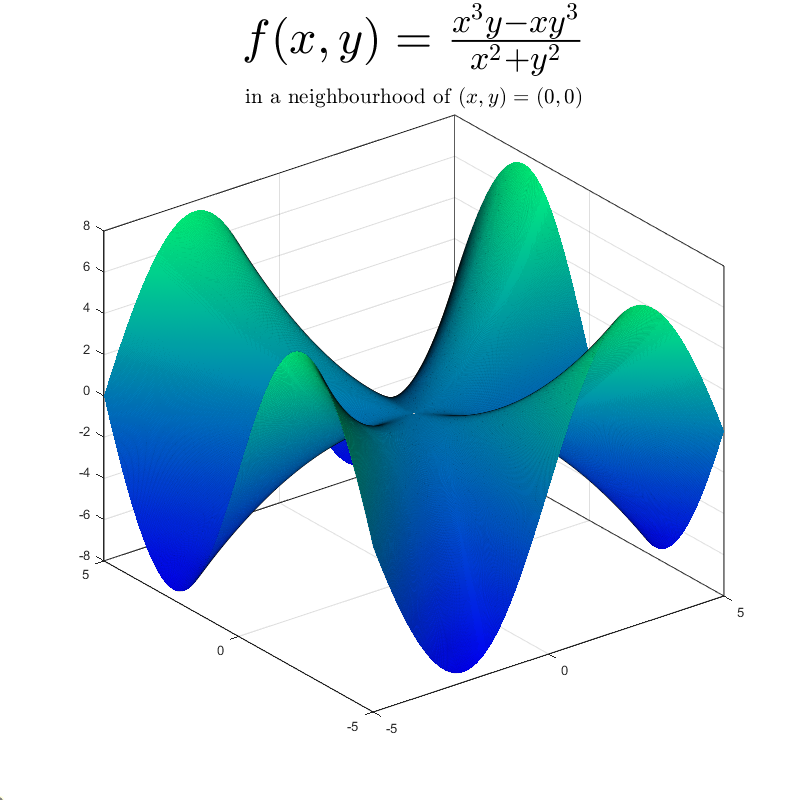
\includegraphics[width=0.6\textwidth]{./PS1_fig1.pdf}
	}
\end{center}

\sol (b)
\begin{align*}
	\cos^3\theta\sin\theta-\cos\theta\sin^3\theta &= \sin\theta\cos\theta(\cos^2\theta-\sin^2\theta) \\
		&= \sin\theta\cos\theta\cos2\theta \\
		&= \bracks{\frac{\sin(\theta+\theta)+\sin(\theta-\theta)}{2}}\cos2\theta \\
		&= \bracks{\frac{\sin(2\theta)+0}{2}}\cos2\theta \\
		&= \frac{1}{2}\sin2\theta\cos2\theta \\
		&= \frac{1}{2}\bracks{\frac{\sin(2\theta+2\theta) + \sin(2\theta-2\theta)}{2}} \\
		&= \frac{1}{2}\bracks{\frac{\sin(4\theta) + \sin(0)}{2}} \\
		&= \frac{1}{4}\sin4\theta \\
	\abs{\sin\theta} &\leq 1 \\
	\abs{\sin4\theta} &\leq 1 \\
	\abs{\frac{1}{4}\sin4\theta} &\leq \frac{1}{4} \\
	\tf\abs{\cos^3\theta\sin\theta-\cos\theta\sin^3\theta} &\leq \frac{1}{4} \\
	\tag*{\QED}
\end{align*}

\sol (c) First, we'll investigate two particular paths, namely $y=0$ and $x=0$.
\begin{multicols}{2}\noindent\begin{align*}
	\lim_{(x,y)\to(0,0)}f(x,0) &= \lim_{(x,y)\to(0,0)}\frac{0-0}{x^2 + 0} \\
		&= \lim_{(x,y)\to(0,0)}\frac{0}{2x} \\
		&= \lim_{(x,y)\to(0,0)}\frac{0}{2} \\
		&= 0 \\
	\lim_{(x,y)\to(0,0)}f(0,x) &= \lim_{(x,y)\to(0,0)}\frac{0-0}{0 + y^2} \\
		&= \lim_{(x,y)\to(0,0)} \frac{0}{2y} \\
		&= \lim_{(x,y)\to(0,0)} \frac{0}{2} \\
		&= 0
\end{align*}\end{multicols}
\noindent These appear to approach a definied limit, 0. \\
\noindent Next, we'll investigate all paths of form $(r,\theta)$,
\begin{align*}
	\lim_{(r,\theta)\to(0,0)}f(r\cos\theta,r\sin\theta) &= \lim_{(r,\theta)\to(0,0)}\frac{r^4\cos^3\theta\sin\theta - r^4\cos\theta\sin^3\theta}{r^2\cos^2\theta + r^2\sin^2\theta} \\
		&= \lim_{(r,\theta)\to(0,0)}\frac{r^4\bracks{\cos^3\theta\sin\theta - \cos\theta\sin^3\theta}}{r^2\bracks{\cos^2\theta + \sin^2\theta}} \\
		&= \lim_{(r,\theta)\to(0,0)}\frac{r^2\bracks{\frac{1}{4}\sin4\theta}}{1} \tag*{(Result from question 3b.)} \\
		&= \lim_{(r,\theta)\to(0,0)}\frac{r^2\sin4\theta}{4} \\
		&= 0\sin0 \\
		&= 0
\end{align*}
So, it seems we've determined the limit exists and is equal to 0.\\
Let's now prove the limit with an $\veps$-$\delta$ proof.
$$
	\lim_{(x,y)\to(a,b)} f(x,y) = L \iff \forall\veps>0,\exists\delta>0: 0 < \sqrt{(x-a)^2+(y-b)^2} < \delta \implies \abs{f(x,y) - L} < \veps.
$$
Namely,
$$
	\lim_{(x,y)\to(0,0)} f(x,y) = 0 \iff \forall\veps>0,\exists\delta>0: 0 < \sqrt{x^2+y^2} < \delta \implies \abs{f(x,y)} < \veps.
$$
Given $\veps > 0$, we choose $\delta = \sqrt{\veps}/2$. Let's suppose $0 < \sqrt{x^2 + y^2} < \delta$.
We can see
\begin{align*}
	\abs{\frac{x^3y - xy^3}{x^2 + y^2}} &= \frac{\abs{xy(x^2 - y^2)}}{x^2 + y^2} \\
		&= \frac{\abs{xy}\abs{x^2 - y^2}}{x^2 + y^2}. \\
	\abs{xy} &= \abs{x}\abs{y}. \\
	\abs{x^2 - y^2} &= \abs{x + y}\abs{x-y} \\
		&\leq \bracks{\abs{x} + \abs{y}}\bracks{\abs{x} + \abs{y}} \\
		&= \bracks{\abs{x} + \abs{y}}^2. \\
	x^2 + y^2 &< \delta^2. \\
	\abs{x} \leq \sqrt{x^2 + y^2} &< \delta. \\
	\abs{y} \leq \sqrt{x^2 + y^2} &< \delta. \\
	\frac{\abs{xy}\abs{x^2 - y^2}}{x^2 + y^2} &\leq \frac{\abs{x}\abs{y}\bracks{\abs{x} + \abs{y}}^2}{x^2 + y^2} \\
		&< \frac{\delta\cd\delta\bracks{\delta + \delta}^2}{\delta^2} \\
		&= \frac{\delta^2\bracks{2\delta}^2}{\delta^2} \\
		&= 4\delta^2 \\
		&= 4\bracks{\frac{\sqrt{\veps}}{2}}^2 \\
		&= 4\bracks{\frac{\veps}{4}} \\
		&= \veps.
\end{align*}
Therefore, we've shown that for all $\veps>0$, we can choose $\delta=\sqrt{\veps}/2$, and if given $0 < \sqrt{x^2+y^2} < \delta$, then $\abs{f(x,y)}<\veps$. So, we've proven that the limit, $\dps{\lim_{(x,y)\to(0,0)}f(x,y)}$, exists and is equal to 0. $\QED$

\end{document}
